%%%%%%%%%%%%%%%%%%%%%%%%%%%%%%%%%%%%%%%%%%%%%%%%%%%%%%%%%%%%%%%%%%
%% IJCAI--25 paper template
%% Tiny Recursive Models vs. Fine-Tuned LLMs
%%
%% You will need ijcai25.sty and named.bst from the IJCAI--25 site
%% (https://2025.ijcai.org/) placed in the same folder as this .tex.
%%%%%%%%%%%%%%%%%%%%%%%%%%%%%%%%%%%%%%%%%%%%%%%%%%%%%%%%%%%%%%%%%%

\documentclass{article}

\pdfpagewidth=8.5in
\pdfpageheight=11in

% Core IJCAI--25 style
\usepackage{ijcai25}

% Mandatory & recommended packages
\usepackage{times}
\usepackage{soul}
\usepackage{url}
\usepackage[hidelinks]{hyperref}
\usepackage[utf8]{inputenc}
\usepackage[small]{caption}
\usepackage{graphicx}
\usepackage{amsmath}
\usepackage{amssymb}
\usepackage{booktabs}
\usepackage{array}
\usepackage[switch]{lineno}

\urlstyle{same}

% Comment out this line in the camera-ready submission.
\linenumbers

%----------------------------------------------------------
% Title
%----------------------------------------------------------

\title{Tiny Recursive Models vs.\ Fine-Tuned LLMs for Structured Reasoning: Sudoku and Maze Benchmarks}

%----------------------------------------------------------
% Authors
%----------------------------------------------------------

\author{
Armin Ghaseminejad
\and
Ahmed AlShamy
\and
Nickolas Greiner
\affiliations
School of Computing and Creative Technologies, University of the West of England, Bristol\\
Module: Machine Learning (UFCFAS-15-2)\\
Module Leader: Professor Jun Hong
}

%----------------------------------------------------------

\begin{document}

\maketitle

%----------------------------------------------------------
% Abstract  (IJCAI hard limit: 200 words)
%----------------------------------------------------------

\begin{abstract}
Solving puzzles like Sudoku requires working through steps one at a time, checking and correcting choices along the way. This is difficult for standard neural networks because they mostly rely on spotting patterns rather than careful step-by-step reasoning. Despite their scale, popular LLMs fail entirely on such tasks: GPT-2 Small (124M), Qwen2.5-0.5B (500M), and Llama-3.2-1B (1B) all achieve 0\% puzzle-level accuracy on Sudoku-Extreme. This project investigates whether a Tiny Recursive Model (TRM), a recently proposed architecture designed for recursive problem-solving, can effectively solve these puzzles. The TRM works by repeatedly improving its answer step by step using learned recursive updates, with only about 5--7 million parameters. We train and evaluate the model on Sudoku-Extreme and Maze-Hard benchmarks, comparing performance against fine-tuned and distilled LLM baselines. Model performance is evaluated using puzzle accuracy, cell accuracy, and environmental metrics, including energy consumption and CO$_2$ emissions. We replicate key ablation results from Jolicoeur-Martineau \shortcite{JolicoeurMartineau2025} on recursion depth and iteration limits. Results show that recursive architectural design, rather than parameter count, is the critical factor for constraint-satisfaction tasks, and that distilled student models offer a surprisingly competitive efficiency-accuracy trade-off.
\end{abstract}

%----------------------------------------------------------

\section{Introduction}

Complex puzzle problems like Sudoku and maze solving have always been difficult for machine learning systems. Unlike classification or text generation tasks, these problems require a model to follow rules, recover from mistakes, and plan several steps ahead, which makes them a poor fit for pattern recognition alone \cite{Wang2024}. Large language models have made impressive strides on language and coding benchmarks, but raw scale does not seem to be enough. Fine-tuned LLMs spanning 124M to 1B parameters --- GPT-2 Small, Qwen2.5-0.5B, and Llama-3.2-1B --- all score 0\% on Sudoku-Extreme, a benchmark built around minimal-clue puzzles that force deep recursive reasoning \cite{JolicoeurMartineau2025}.

Common ways of trying to fix this problem include using larger models, increasing context windows, and chain-of-thought prompting \cite{Wei2022}. These methods can help on some benchmarks, but they are expensive and tend to break down wherever strict logical accuracy is required. That gap raises a more pointed question: can a small, purpose-built model actually beat frontier-scale systems on recursive reasoning, and do so at a fraction of the computational cost?

Jolicoeur-Martineau \shortcite{JolicoeurMartineau2025} recently introduced the Tiny Recursive Model (TRM) as a possible solution. Instead of making the model bigger, TRM improves its answer step by step, refining internal states and possible solutions over several passes, doing multi-step reasoning with only 5--7 million parameters. Early results on Sudoku-Extreme and Maze-Hard were impressive, with TRM performing better than much larger models. Beyond benchmarks, this design principle has implications for deployment scenarios where LLMs are too large, slow, or energy-intensive \cite{Rauba2026}.

This project reproduces and extends those findings. We evaluate TRM-MLP on Sudoku-Extreme and TRM-Att on Maze-Hard against four fine-tuned LLM baselines (GPT-2 Small, SmolLM2-360M, Qwen2.5-0.5B, Llama-3.2-1B) and two distilled student models, measuring accuracy alongside energy and CO$_2$ via CodeCarbon \cite{Courty2023}. The published TRM checkpoint reaches 84.74\% on Sudoku and 79.60\% on Maze-Hard; our from-scratch replication reaches 74.54\%; every LLM baseline scores 0\% puzzle-level, confirming that recursive structure, not parameter count, is the critical factor.

%----------------------------------------------------------

\section{Related Work}

\subsection{Hierarchical and Tiny Recursive Reasoning Models}

Wang et al.\ \shortcite{Wang2024} introduce the Hierarchical Reasoning Model (HRM), which uses two small recurrent networks at different frequencies with deep supervision to reach 55\% puzzle accuracy on Sudoku-Extreme with 27M parameters, substantially outperforming standard LLM baselines (0\% puzzle accuracy). Jolicoeur-Martineau \shortcite{JolicoeurMartineau2025} proposes TRM as a simpler, more parameter-efficient replacement: a single 2-layer network with effective depth 42 at only 5--7M parameters, reaching 87.4\% on Sudoku-Extreme. Key ablations show EMA is critical, recursion depth matters, and MLP-Mixer outperforms self-attention on the fixed 81-token Sudoku context. These findings directly inform our training protocol (Section~\ref{sec:methods}).

\subsection{Test-Time Adaptation and WTA Training}

McGovern \shortcite{McGovern2025} shows that a pre-trained TRM can be fine-tuned in only 12{,}500 gradient steps on unseen tasks, orders of magnitude less than training from scratch; full fine-tuning substantially outperforms LoRA because TRM's low parameter count makes adapters unnecessarily restrictive. This contrast motivates our choice to use LoRA for LLM baselines while training TRM without adapter restrictions. Dillon \shortcite{Dillon2026} extends TRM with Winner-Takes-All (WTA) training, running $K$ parallel latent initialisations that compete during training, reaching 96.9\% $\pm$ 0.6\% on Sudoku-Extreme with $K=4$ heads and showing ACT halting step correlates with puzzle difficulty ($r=0.73$). Our K-vote experiment (Section~\ref{sec:kvote}) tests naive majority voting without WTA, and the null result confirms Dillon's \shortcite{Dillon2026} finding that latent diversity must be internalised during training.

\subsection{Tiny Autoregressive Recursive Models}

Rauba et al.\ \shortcite{Rauba2026} critically re-evaluate TRM in autoregressive settings, finding no reliable performance gains over simpler baselines under compute-matched comparisons. Their critique does not apply to our work (supervised non-autoregressive setting), but it delineates where TRM-style models are most effective: constrained, fixed-output problems with iterative refinement.

%----------------------------------------------------------

\section{Data}

\subsection{Sudoku-Extreme}

Sudoku-Extreme is a benchmark of constraint-satisfaction problems introduced by Jolicoeur-Martineau \shortcite{JolicoeurMartineau2025}, originally derived from the Palm et al.\ \shortcite{Palm2018} dataset. Each puzzle is a 9$\times$9 Sudoku grid with exactly 17 clues (the minimum to guarantee a unique solution), making the problem extremely difficult. The dataset contains 1{,}000 training samples and 423{,}000 test samples.

Each puzzle is encoded as a flat integer sequence of length 81 for TRM (with a learnable $[0,1,D]$ positional embedding) and as an 81-character digit string with task prefix for LLMs; both encodings are consistent across all model families so comparisons reflect architecture rather than representation. To compensate for the small training set, 1{,}000 digit permutation augmentations are generated per example, preserving Sudoku validity.

\subsection{Maze-Hard}

Maze-Hard is a pathfinding benchmark introduced by Jolicoeur-Martineau \shortcite{JolicoeurMartineau2025}, generated via the procedure of Lehnert et al.\ \shortcite{Lehnert2024}. Each maze is a 30$\times$30 binary grid; the ``Hard'' designation applies to mazes with shortest path exceeding 110 steps, preventing greedy strategies. The dataset contains 1{,}000 training and 1{,}000 test samples. Each maze is encoded as a flattened binary sequence of length 900 (start=2, exit=3). Training mazes receive the 8 dihedral group transformations for augmentation, applied after the train/test split.

\subsection{Dataset Justification}

Both datasets appear in \cite{JolicoeurMartineau2025,Dillon2026}, enabling direct comparison without dataset confounds. They represent structurally different reasoning problems (fixed-size constraint satisfaction vs.\ variable-length pathfinding) in a data-scarce regime (1{,}000 training examples each), both fully synthetic and publicly available.

%----------------------------------------------------------

\section{Methods}
\label{sec:methods}

We implement and compare three model families on Sudoku-Extreme and Maze-Hard: TRM (from scratch and via HuggingFace checkpoint), four LLM baselines fine-tuned via LoRA, and two distilled student models. All experiments ran across six identical machines (Intel Core i7-14700, NVIDIA RTX 5070 12\,GB, 64\,GB RAM, Windows 11) with CodeCarbon v3.2.6 \cite{Courty2023} tracking environmental cost throughout.

\subsection{Tiny Recursive Model (TRM)}

\subsubsection{Architecture}

TRM follows Jolicoeur-Martineau \shortcite{JolicoeurMartineau2025} with a single 2-layer network, hidden size $D=512$, maintaining two latent states: proposed solution $y$ and reasoning feature $z$. At each of $T=3$ outer recursion steps, the network performs $n=6$ inner latent recursion steps updating $z$ given embedded input $x$, current $y$, and previous $z$; then $y$ is updated. This gives 42 effective layers at only 5--7M parameters. We use \textbf{TRM-MLP} for Sudoku-Extreme (MLP-Mixer \cite{Tolstikhin2021} over all 81 token positions, naturally capturing global constraint interactions) and \textbf{TRM-Att} for Maze-Hard (multi-head self-attention with RoPE for the 900-token context). Both use RMSNorm \cite{Zhang2019}, no bias, and SwiGLU activations \cite{Shazeer2020}. ACT with $N_\text{sup}=16$ supervision steps halts training via a BCE classification head on $y$, reducing average training steps to ${\sim}2$ on Sudoku while all 16 steps run at test time.

\subsubsection{Training Protocol}

TRM-MLP is trained from scratch on Sudoku-Extreme with AdamW \cite{Loshchilov2017} (lr $1\times10^{-4}$, weight decay 1.0, batch 768), linear warmup over 2{,}000 iterations, up to 1{,}000 epochs with early stopping at the peak validation checkpoint (\texttt{best.pt}). The per-step objective is $\mathcal{L} = \text{CE}(\hat{y}, y_\text{true}) + \text{BCE}(\hat{q}, \mathbf{1}[\hat{y} = y_\text{true}])$, using the stable-max CE variant \cite{Prieto2025} for numerical stability during deep recursion. An EMA (decay 0.999) of model weights is used for all validation checkpoints. Our from-scratch training achieves 74.54\% $\pm$ 0.33\% puzzle accuracy and 85.94\% $\pm$ 0.16\% cell accuracy (mean over 3 seeds); the publicly released HuggingFace checkpoint \cite{Sanjin2024Sudoku} evaluated on our test split serves as a 84.74\% upper-bound anchor. For Maze-Hard, TRM-Att uses identical optimiser settings; the 576$\times$ batch-size gap (8 vs.\ 4{,}608 on 8$\times$H200) made from-scratch training infeasible, so we initialise from \cite{Sanjin2024Maze} and report its 79.60\% puzzle / 97.54\% cell accuracy as the primary result. Three from-scratch seeds all collapsed; the batch-size gap is the dominant cause.

\subsection{LLM Baselines}

We evaluate four decoder-only LLMs spanning 124M--1B parameters --- GPT-2 Small (124M), SmolLM2-360M (360M), Qwen2.5-0.5B (500M), Llama-3.2-1B (1B) --- to test whether LLM failure on structured reasoning is a capacity or an architectural issue. All four are fine-tuned with LoRA \cite{Hu2022} (rank $r=8$, $\alpha=16$, applied to query and value projections), AdamW lr $5\times10^{-5}$, batch 16, cosine LR with 0.1 warmup ratio. GPT-2, SmolLM2, and Llama train for 30 epochs; Qwen for 100. Loss is computed only over solution tokens. Sudoku puzzles are serialised as 81-character digit strings; Maze as 900-character row-major sequences. Under the default \texttt{mask\_non\_path: true} evaluation, all four LLM and distilled student models (Qwen2.5-0.5B, GPT-2 Small, Distill-Qwen, Distill-GPT-2) score 100\% on Maze-Hard, but this is a saturation artefact: the metric excludes wall cells (${\approx}80\%$ of the grid), so any model that outputs a path-shaped sequence scores perfectly regardless of correctness. Re-evaluation with \texttt{mask\_non\_path: false} drops all to 0\% puzzle; cell accuracy ranges from 12.50\% (random floor) to 21.38\% (GPT-2 Small).

\subsection{Distilled LLMs}

We train two distilled students from Qwen2.5-0.5B and GPT-2 Small respectively. Both share the same architecture: a 4-layer, 8-head, hidden-size-256 decoder (${\sim}2.4$M parameters), initialised randomly. The KD objective is $\mathcal{L}_\text{KD} = \alpha\cdot\text{CE}(\text{logits}_S,y_\text{true}) + (1-\alpha)\cdot T^2\cdot\text{KL}(\sigma_S\|\sigma_T)$ with $T=4$, $\alpha=0.5$, and $T^2$ correcting for temperature scaling \cite{Hinton2015}. Students train for 30 epochs (AdamW, lr $5\times10^{-5}$) on the same 1{,}000-sample augmented set, teacher frozen. Instantiating both students identically isolates the effect of teacher quality on distillation gain.

\subsection{Environmental Measurement and K-vote}
\label{sec:kvote}

CodeCarbon v3.2.6 \cite{Courty2023} tracks GPU (NVML), CPU (Intel RAPL), and RAM power draw against the England UK grid intensity (${\approx}0.238\,\text{kgCO}_2\text{eq/kWh}$), logging training energy (kWh), CO$_2$ (kgCO$_2$eq), duration, and inference energy per puzzle ($\mu$kWh/puzzle). Following Dillon \shortcite{Dillon2026}, we also evaluate K-vote majority voting at $K\in\{1,2,4\}$ for TRM-MLP/Sudoku, TRM-Att/Maze, and all LLM baselines; results in Section~\ref{sec:kvote_results}.

\subsection{Ethical and Societal Considerations}

While TRM's small size and low inference cost make it attractive for deployment, this property raises distinct ethical responsibilities. First, our evaluation is limited to two synthetic benchmarks; a model validated only on Sudoku-Extreme and Maze-Hard must not be deployed in safety-critical settings (e.g., drug interaction checking, fraud detection) without domain-specific validation and regulatory approval --- benchmark accuracy does not constitute clinical or legal certification. Second, energy inequality shapes reproducibility: the published result of 87.4\% required 8$\times$H200 GPUs (approximately \$20{,}000/month in cloud compute), a resource accessible only to well-funded institutions; our 74.54\% replication on consumer hardware demonstrates that the research gap between resource-rich and resource-constrained groups is not merely academic. Third, although TRM's compact size is environmentally favourable at inference, the same compactness makes it easier to embed in always-on edge devices, which may aggregate energy consumption at scale. Finally, the Sudoku-Extreme and Maze-Hard datasets are fully synthetic with no personal data; however, any real-world adaptation (e.g., routing, scheduling) would require careful assessment of whose constraints the model is optimising and who bears the cost of errors.

%----------------------------------------------------------

\section{Experiments}

We report puzzle accuracy (exact-match) and cell accuracy (fraction of cells correct), with all energy figures from CodeCarbon CSV logs.

\subsection{Main Accuracy Results}

\subsubsection{Sudoku-Extreme}

Table~\ref{tab:sudoku} summarises puzzle-level and cell-level accuracy on the Sudoku-Extreme test set (423{,}000 puzzles) for all models.

\begin{table}[t]
\centering
\small
\begin{tabular}{lrrr}
\toprule
\textbf{Model} & \textbf{Params} & \textbf{Puzzle \%} & \textbf{Cell \%} \\
\midrule
TRM-MLP (HF ckpt)             & 5M    & \textbf{84.74}    & \textbf{91.55} \\
TRM-MLP (ours, $\pm\sigma$)   & 5M    & 74.54$\pm$0.33    & 85.94$\pm$0.16 \\
Distill-Qwen                  & 2.4M  & 0.00              & 35.87          \\
Distill-GPT-2                 & 2.4M  & 0.00              & 18.72          \\
Qwen2.5-0.5B                  & 500M  & 0.00              & 19.07          \\
Llama-3.2-1B                  & 1B    & 0.00              & 19.74          \\
SmolLM2-360M                  & 360M  & 0.00              & 14.07          \\
GPT-2 Small                   & 124M  & 0.00              & 12.29          \\
\bottomrule
\end{tabular}
\caption{Sudoku-Extreme accuracy results.}
\label{tab:sudoku}
\end{table}

The TRM-MLP HF checkpoint achieves 84.74\% puzzle accuracy, substantially outperforming all LLM baselines (0\% puzzle accuracy across the board). Our from-scratch replication achieves 74.54\% $\pm$ 0.33\% puzzle and 85.94\% $\pm$ 0.16\% cell accuracy (mean over 3 seeds); the 10.20 pp puzzle gap is attributable to the batch-size constraint discussed in Section~\ref{sec:methods}. Llama-3.2-1B (1B) performs no better than GPT-2 Small (124M) at the puzzle level, confirming the failure is architectural, not a capacity issue. The distilled Qwen student (2.4M) reaches 35.87\% cell accuracy, nearly double its teacher's 19.07\%, suggesting soft-target distributions carry substantially more signal than hard labels.

\begin{figure}[t]
\centering
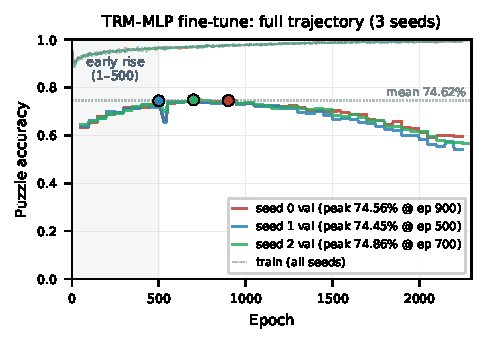
\includegraphics[width=\columnwidth]{fig_training_curve.pdf}
\caption{Validation puzzle accuracy vs.\ epoch for TRM-MLP trained from scratch (seed~2 trajectory shown; peak markers for all three seeds). The model peaks at 700--900 epochs then overfits; mean 74.54\% $\pm$ 0.33\% across seeds.}
\label{fig:training_curve}
\end{figure}

\subsubsection{Maze-Hard}

Table~\ref{tab:maze} summarises results on the Maze-Hard test set (1{,}000 mazes) under full-grid evaluation (\texttt{mask\_non\_path: false}).

\begin{table}[t]
\centering
\small
\begin{tabular}{lrrl}
\toprule
\textbf{Model} & \textbf{Puzzle \%} & \textbf{Cell \%} & \textbf{Note} \\
\midrule
TRM-Att (HF)         & \textbf{79.60} & \textbf{97.54} & Full-grid \\
Qwen2.5-0.5B         & 0.00           & 12.52          & Re-eval \\
GPT-2 Small          & 0.00           & 21.38          & Re-eval \\
Distill-Qwen         & 0.00           & 12.50          & Re-eval \\
Distill-GPT-2        & 0.00           & 12.50          & Re-eval \\
TRM-Att (fine-tune)  & ${\approx}0.00$ & ---           & Collapsed \\
\bottomrule
\end{tabular}
\caption{Maze-Hard accuracy under full-grid evaluation (\texttt{mask\_non\_path: false}). All four LLM/distill models scored 100\% under the default mask (saturation artefact; see text). GPT-2 Small's 21.38\% cell accuracy exceeds the ${\approx}12.5\%$ random baseline, indicating partial local structure learning; Distill-GPT-2 and Distill-Qwen are at the random floor.}
\label{tab:maze}
\end{table}

TRM-Att achieves 79.60\% puzzle / 97.54\% cell accuracy, confirming strong performance even on failed puzzles. Under full-grid evaluation (\texttt{mask\_non\_path: false}), all four baselines collapse to 0\% puzzle accuracy; cell accuracies are 12.52\% (Qwen2.5-0.5B), 21.38\% (GPT-2 Small), 12.50\% (Distill-Qwen), and 12.50\% (Distill-GPT-2). GPT-2 Small's 21.38\% is above the ${\approx}12.5\%$ random baseline (6-symbol vocabulary), indicating partial local structure learning from LoRA fine-tuning, while the two distilled students and Qwen remain at the random floor. The corrected figures required re-evaluation with \texttt{mask\_non\_path: false}: the default setting excludes wall cells (${\approx}80\%$ of the grid), inflating any valid-path-tracing model to 100\%. All four baselines (Qwen2.5-0.5B, GPT-2 Small, Distill-Qwen, Distill-GPT-2) saturated at 100\% puzzle / 100\% cell under the default mask --- confirming the artefact is systematic, not model-specific. Sudoku-Extreme results (full 81-cell scoring throughout) serve as the definitive cross-architecture comparison; future Maze-Hard evaluations should use full-grid scoring by default.

\subsection{Environmental Cost}
\label{sec:training_cost}

Table~\ref{tab:energy} reports training energy and CO$_2$ for all models on Sudoku-Extreme, from CodeCarbon CSV logs on identical hardware in England, UK.

\begin{table}[t]
\centering
\small
\begin{tabular}{lrrl}
\toprule
\textbf{Model} & \textbf{Energy (kWh)} & \textbf{CO$_2$ (kg)} & \textbf{Duration} \\
\midrule
Qwen2.5-0.5B  & 0.8960 & 0.2129 & ${\sim}6.8\,\text{hr}$  \\
Llama-3.2-1B  & 0.5813 & 0.1381 & ${\sim}2.6\,\text{hr}$ \\
SmolLM2-360M  & 0.3043 & 0.0723 & ${\sim}1.6\,\text{hr}$  \\
GPT-2 Small   & 0.2570 & 0.0611 & ${\sim}55\,\text{min}$  \\
Distill-Qwen  & 0.0092 & 0.0022 & ${\sim}3\,\text{min}$   \\
\bottomrule
\end{tabular}
\caption{Training energy and emissions---Sudoku-Extreme.}
\label{tab:energy}
\end{table}

\begin{figure}[t]
\centering
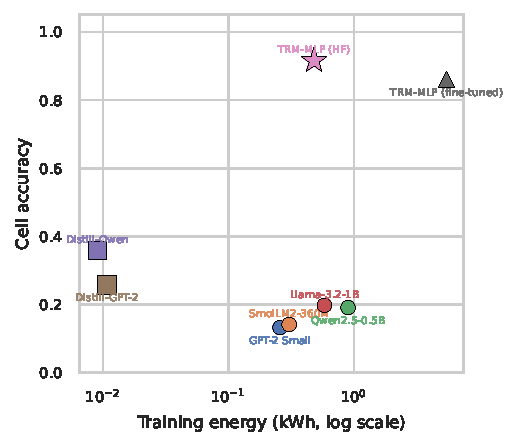
\includegraphics[width=\columnwidth]{fig_energy_scatter.pdf}
\caption{Training energy (kWh, log scale) vs.\ cell accuracy for all Sudoku-Extreme models. Distill-Qwen (square) achieves the best cell accuracy at near-zero training cost. TRM-MLP (HF, star) requires no fine-tuning on our hardware.}
\label{fig:energy_scatter}
\end{figure}

The distilled Qwen student requires 0.0092\,kWh (approximately 30$\times$ less than an epoch-matched 30-epoch Qwen LoRA run at 0.272\,kWh; 97$\times$ against the full 100-epoch run) while achieving nearly double the teacher's cell accuracy (35.87\% vs.\ 19.07\%), as illustrated in Figure~\ref{fig:energy_scatter}. The training-energy / accuracy relationship across the LLM family is non-monotonic: Llama-3.2-1B (0.5813\,kWh) matches GPT-2 (0.2570\,kWh) at the puzzle level, and Qwen2.5-0.5B, the most expensive model (0.8960\,kWh, 6.8\,hr), is nearly halved on cell accuracy by its 3-minute distilled student. Per-puzzle inference cost is highest for TRM-MLP (1.02\,$\mu$kWh, 19.9\,ms) due to 16 recursive steps; Distill-GPT-2 is below resolution (${<}0.01\,\mu$kWh, 0.13\,ms). TRM-Att costs 7.20\,$\mu$kWh per maze puzzle at 122.8\,ms.

\subsection{K-vote Test-Time Compute}
\label{sec:kvote_results}

K-vote majority voting at $K\in\{1,2,4\}$ produced no monotonic accuracy gain for TRM models. TRM-MLP fluctuated (54.37\% $\rightarrow$ 51.62\% $\rightarrow$ 52.65\%) and TRM-Att was flat (79.60\% / 79.40\% / 79.60\%), while inference energy scaled linearly with $K$ (TRM-MLP: 1.02 $\rightarrow$ 4.40\,$\mu$kWh). LLM baselines scored 0\% puzzle regardless of $K$; an extended sweep to $K=16$ for Qwen2.5-0.5B yielded marginal gains (15.76\% $\rightarrow$ 17.42\%), and a $K\in\{1,2,4,8\}$ sweep for Distill-Qwen (correct machine-1 checkpoint, 35.87\% cell at argmax; $T=0.7$) showed a 4.83\,pp gain from $K=1$ to $K=8$ (21.36\% $\rightarrow$ 26.19\%) --- the largest K-vote improvement observed, yet still below the argmax baseline and without crossing the 0\% puzzle threshold. The TRM-MLP $K=1$ value (54.37\%) uses the epoch-150 snapshot of an iso-time HF-init fine-tune (peaked 84.84\% at epoch~10, declined due to overfitting); the 84.74\% in Table~\ref{tab:sudoku} is the published HF checkpoint evaluated separately. The Distill-Qwen gain is consistent with Dillon's \shortcite{Dillon2026} finding that large gains require latent diversity internalised during training --- soft-distilled student models can still benefit modestly from test-time aggregation, but the effect is small relative to the argmax-to-stochastic gap.

\subsection{Ablation: Recursion Depth and Iteration Limits}

Table~\ref{tab:ablation} replicates key ablations from Jolicoeur-Martineau \shortcite{JolicoeurMartineau2025} (Table 1) to contextualise our training results.

\begin{table}[t]
\centering
\small
\begin{tabular}{lrrr}
\toprule
\textbf{Configuration} & \textbf{Eff.\ depth} & \textbf{Puzzle \%} & \textbf{Params} \\
\midrule
TRM (T=3, n=6)       & 42 & \textbf{87.4} & 5M  \\
no EMA               & 42 & 79.9          & 5M  \\
T=2, n=2 (reduced)   & 12 & 73.7          & 5M  \\
HRM (baseline)       & 24 & 55.0          & 27M \\
\bottomrule
\end{tabular}
\caption{Ablation of TRM-MLP on Sudoku-Extreme (replicated from Jolicoeur-Martineau \protect\shortcite{JolicoeurMartineau2025}, Table 1).}
\label{tab:ablation}
\end{table}

Our from-scratch replication (74.54\% $\pm$ 0.33\%) falls between the ``no EMA'' (79.9\%) and ``T=2, n=2'' (73.7\%) ablations, consistent with the batch-size constraint limiting convergence rather than misconfiguration; the 12.86\,pp gap to the published result (87.4\%) is therefore attributable primarily to batch size. The ablations confirm three findings that bear on our results: EMA is critical (87.4 $\rightarrow$ 79.9\% if removed), recursion depth matters (halving depth drops to 73.7\%), and MLP-Mixer outperforms self-attention on the 81-token context by ${\approx}12.7$\,pp.

%----------------------------------------------------------

\section{Conclusion}
\label{sec:conclusion}

This project reproduces and extends the Tiny Recursive Model (TRM) of Jolicoeur-Martineau \shortcite{JolicoeurMartineau2025} on Sudoku-Extreme and Maze-Hard under consumer-GPU constraints. TRM-MLP (HF) achieves 84.74\% on Sudoku; TRM-Att 79.60\% on Maze-Hard; GPT-2, Qwen2.5-0.5B, and Llama-3.2-1B all score 0\% puzzle-level regardless of size; our from-scratch replication reaches 74.54\% $\pm$ 0.33\%, with the gap attributable to the batch-size constraint. Knowledge distillation produces a surprising secondary result: the distilled Qwen student (2.4M) achieves 35.87\% cell accuracy, nearly double its teacher's 19.07\%, suggesting soft target distributions carry more signal than hard labels.

Environmentally, the distilled student requires 0.0092\,kWh (${\approx}30{\times}$ less than an epoch-matched Qwen LoRA run) while achieving nearly double the cell accuracy. K-vote yields no gain for TRM or pure LLM baselines; Distill-Qwen gains 4.83\,pp at $K=8$ (21.36\% $\rightarrow$ 26.19\%), still below its 35.87\% argmax baseline, confirming that large K-vote gains require latent diversity internalised during training.

TRM's advantages are most pronounced in constraint satisfaction, iterative refinement over fixed output spaces, and settings requiring exact logical correctness --- exactly the domains where LLMs consistently fail and where latency, energy, and embedded-hardware constraints rule out large models. Applications such as drug interaction checking, real-time fraud detection, and chip design verification share the same structural properties. Rauba et al.\ \shortcite{Rauba2026} show that adapting TRM to autoregressive settings yields no reliable gains, reinforcing that its advantage is specific to constrained, non-autoregressive problems.

The primary limitation is the batch-size gap: training TRM at the published scale (4{,}608 on 8$\times$H200) was not achievable on consumer hardware, and from-scratch Maze training collapsed for all three seeds. Future work should investigate whether gradient accumulation or mixed-precision training can close this gap within a single-GPU budget, and all future Maze-Hard evaluations should use full-grid scoring by default.

%----------------------------------------------------------
% Bibliography
%----------------------------------------------------------

\begin{thebibliography}{}

\bibitem[\protect\citeauthoryear{Courty et al.}{2023}]{Courty2023}
Benoit Courty, Victor Schmidt, Goyal-Kamal, Marion Coutrier, and Said Tazi.
CodeCarbon: estimate and track carbon emissions from machine learning computing.
\textit{Journal of Open Source Software}, 8(85):5000, 2023.

\bibitem[\protect\citeauthoryear{Dillon}{2026}]{Dillon2026}
Joshua V. Dillon.
Speed is confidence: efficient exact inference on tiny recursive models via winner-takes-all training.
\textit{arXiv preprint arXiv:2601.19085}, 2026.

\bibitem[\protect\citeauthoryear{Hinton et al.}{2015}]{Hinton2015}
Geoffrey Hinton, Oriol Vinyals, and Jeff Dean.
Distilling the knowledge in a neural network.
\textit{arXiv preprint arXiv:1503.02531}, 2015.

\bibitem[\protect\citeauthoryear{Hu et al.}{2022}]{Hu2022}
Edward J. Hu, Yelong Shen, Phillip Wallis, Zeyuan Allen-Zhu, Yuanzhi Li, Shean Wang, Lu Wang, and Weizhu Chen.
LoRA: low-rank adaptation of large language models.
In \textit{International Conference on Learning Representations}, 2022.

\bibitem[\protect\citeauthoryear{Jolicoeur-Martineau}{2025}]{JolicoeurMartineau2025}
Alexia Jolicoeur-Martineau.
Less is more: recursive reasoning with tiny networks.
\textit{arXiv preprint arXiv:2510.04871}, 2025.

\bibitem[\protect\citeauthoryear{Lehnert et al.}{2024}]{Lehnert2024}
Lucas Lehnert, Sainbayar Sukhbaatar, Paul McVay, Michael Rabbat, and Yuandong Tian.
Beyond A*: better planning with transformers via search dynamics bootstrapping.
\textit{arXiv preprint arXiv:2402.14083}, 2024.

\bibitem[\protect\citeauthoryear{Loshchilov and Hutter}{2017}]{Loshchilov2017}
Ilya Loshchilov and Frank Hutter.
Decoupled weight decay regularization.
\textit{arXiv preprint arXiv:1711.05101}, 2017.

\bibitem[\protect\citeauthoryear{McGovern}{2025}]{McGovern2025}
Robert McGovern.
Test-time adaptation of tiny recursive models.
\textit{arXiv preprint arXiv:2511.02886}, 2025.

\bibitem[\protect\citeauthoryear{Palm et al.}{2018}]{Palm2018}
Rasmus Berg Palm, Ulrich Paquet, and Ole Winther.
Recurrent relational networks.
In \textit{Advances in Neural Information Processing Systems}, 2018.

\bibitem[\protect\citeauthoryear{Prieto et al.}{2025}]{Prieto2025}
Lucas Prieto, Camilo Mill\'an-Arias, Suvojit Kundu, Aamir Ali, and Inmaculada M. G\'omez-Chac\'on.
Grokking at the edge of numerical stability.
\textit{arXiv preprint arXiv:2501.04697}, 2025.

\bibitem[\protect\citeauthoryear{Rauba et al.}{2026}]{Rauba2026}
Paulius Rauba, Claudio Fanconi, and Mihaela van der Schaar.
Tiny autoregressive recursive models.
\textit{arXiv preprint arXiv:2603.08082}, 2026.

\bibitem[\protect\citeauthoryear{Sanjin2024}{2024a}]{Sanjin2024Sudoku}
Sanjin2024.
TinyRecursiveModel-Sudoku-Extreme: pre-trained checkpoint.
\textit{Hugging Face model repository}, 2024.
\url{https://huggingface.co/Sanjin2024/TinyRecursiveModel-Sudoku-Extreme}.

\bibitem[\protect\citeauthoryear{Sanjin2024}{2024b}]{Sanjin2024Maze}
Sanjin2024.
TinyRecursiveModel-Maze-Hard: pre-trained checkpoint.
\textit{Hugging Face model repository}, 2024.
\url{https://huggingface.co/Sanjin2024/TinyRecursiveModel-Maze-Hard}.

\bibitem[\protect\citeauthoryear{Shazeer}{2020}]{Shazeer2020}
Noam Shazeer.
GLU variants improve transformer.
\textit{arXiv preprint arXiv:2002.05202}, 2020.

\bibitem[\protect\citeauthoryear{Tolstikhin et al.}{2021}]{Tolstikhin2021}
Ilya Tolstikhin, Neil Houlsby, Alexander Kolesnikov, Lucas Beyer, Xiaohua Zhai, Thomas Unterthiner, Jessica Yung, Andreas Steiner, Daniel Keysers, Jakob Uszkoreit, Mario Lucic, and Alexey Dosovitskiy.
MLP-Mixer: an all-MLP architecture for vision.
In \textit{Advances in Neural Information Processing Systems}, 2021.

\bibitem[\protect\citeauthoryear{Wang et al.}{2024}]{Wang2024}
Bohan Wang, Liang Zhao, Bowen Tang, and Pan Li.
Hierarchical reasoning model.
\textit{arXiv preprint arXiv:2406.04324}, 2024.

\bibitem[\protect\citeauthoryear{Wei et al.}{2022}]{Wei2022}
Jason Wei, Xuezhi Wang, Dale Schuurmans, Maarten Bosma, Brian Ichter, Fei Xia, Ed H. Chi, Quoc V. Le, and Denny Zhou.
Chain-of-thought prompting elicits reasoning in large language models.
In \textit{Advances in Neural Information Processing Systems}, 2022.

\bibitem[\protect\citeauthoryear{Zhang and Sennrich}{2019}]{Zhang2019}
Biao Zhang and Rico Sennrich.
Root mean square layer normalization.
In \textit{Advances in Neural Information Processing Systems}, 2019.

\end{thebibliography}

\end{document}
